\section{Исследование и построение решения задачи}
\label{sec:Chapter3} \index{Chapter3}

Рассмотрим все компоненты люстры и обратим внимание на те места, где может образоваться бутылочное горлышко.

\subsection{Устройство параллельной файловой системы Lustre}

\begin{figure}[h]
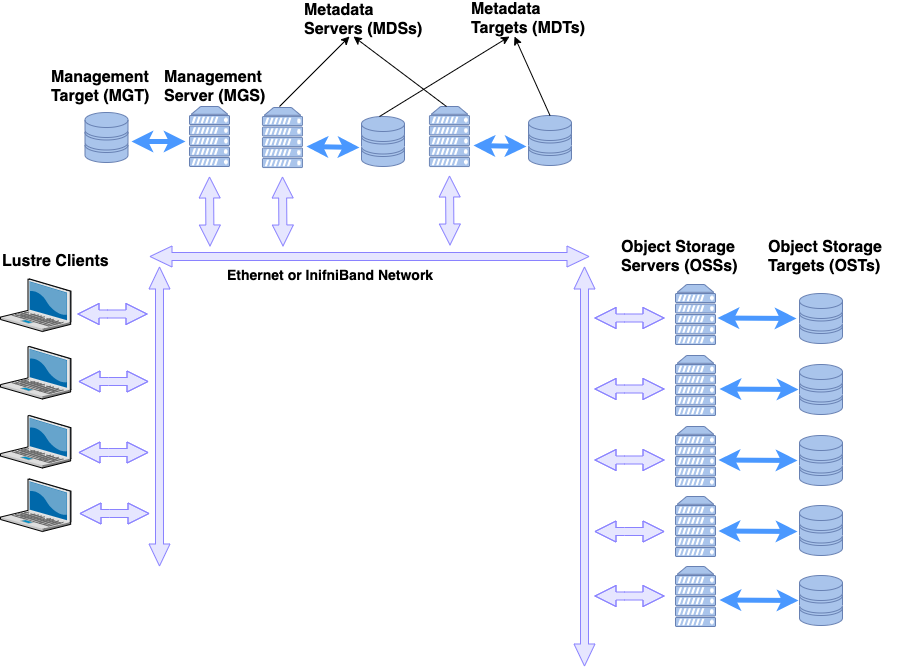
\includegraphics[height=12.5cm,keepaspectratio]{./lustre_components.png}\\[0.1cm]
\caption{Основные компоненты файловой системы Lustre}
\label{lustre_components}
\end{figure}

Существуют сервера управления и подконтрольные им сервера, которые называются соответственно Server и Target. 


MDS(Metadata Server) --- эти сервера отвечают за все операции над пространствами имён всей файловой системы Lustre. Вся информация
об иерархии директорий и метаданных файлов хранится на Target серверах, а MDS предоставляет логический интерфейс
для этих данных. В файловой системе всегда есть как минимум один MDS и соответствующий ему MDT, серверов второго 
типа может быть добавлено больше, чтобы удовлетворить запросы конкретной среды. Сервера метаданных управляют
распределением объектов хранения между серверами OSS для содержимого при создании файлов, а также управляют 
открытием и закрытием файлов, их удалением и переименованием и другими операциями над пространствами имён.

А на серверах MDT (Metadata Target) фактически хранится вся метаинформация пространства имён, такая как имена файлов, директорий,
права доступа, расположение файлов и индексы данных для эффективного доступа к хранимым в файловой системе данным.
Возможность иметь несколько MDT в одной файловой системе позволяет поддеревьям каталогов храниться на вторичном
MDT, что очень полезно для изоляции рабочих нагрузок, которые особенно интенсивно потребляют метаданные на
выделенном оборудовании (например, отдельный сервер MDT может быть выделен для определённого набора проектов).
Большие каталоги могут быть распределены по нескольким MDT, обеспечивая масштабируемость для приложений,
которые генерируют очень большое количество файлов в плоской иерархии директорий (множество файлов хранится в одной директории, а не разделяется между несколькими).

OSS(Object Storage Server) обеспечивает массовое хранение содержимого файлов в файловой системе Lustre. Один или несколько серверов хранения
данных OSS хранят данные файлов на одном или нескольких OST (Object Storage Target), в одной файловой системе Lustre могут быть тысячи 
серверов OSS. Обычно один OSS обслуживает от двух до восьми серверов OST (хотя возможно намного больше).
Ёмкость файловой системы Lustre это сумма всех ёмкостей, предоставляемых серверами хранения данных OSS через сервера OST.
OSS обычно конфигурируются парами, причём каждая пара подключается к общему внешнему хранилищу, которая
хранит сервера OST. Данный пример можно увидеть на рисунке~\ref{lustre_components}
Сервера OST доступны через два сервера в конфигурации активной и пассивной отказоустойчивости
для поддержания высокой доступности даже в случае каких-либо сбоев. OST монтируются только на одном сервере
одновременно и обычно равномерно распределены между всеми OSS для балансирования производительности и
максимизации пропускной способности.


MGS(Management Server) --- сервер управления, он хранит всю информацию о конфигурациях для всех файловых систем Lustre в кластере и
предоставляет эту информацию другим хостам Lustre. Сервера и клиенты подключаются именно к MGS при запуске,
чтобы получить конфигурации файловой системы. Уведомления обо всех изменениях в конфигурациях файловой системы,
включая перезагрузки серверов, распространяются именно MGS.
Постоянная информация для всех узлов кластера запоминается и записывается на устройства хранения, называемые MGT (Management Target).
MGS может быть совмещён с сервером MDS в конфигурации с очень высокой доступностью, при этом каждый сервер
подключен к общему хранилищу. Несколько файловых систем Lustre могут управляться только одним MGS.


Клиенты --- приложения получают доступ к данным файловой системы и используют их, взаимодействуя с клиентами Lustre.
Клиент Lustre представлен в виде точки монтирования файловой системы на хосте и предоставляет приложениям единое
пространство имен для всех файлов и данных в файловой системе, используя стандартную семантику POSIX. Файловая
система Lustre, установленная в клиентской операционной системе, очень похожа на любую другую файловую систему
POSIX; каждый экземпляр Lustre представлен как отдельная точка монтирования в операционной системе клиента, и
каждый клиент может монтировать несколько разных экземпляров файловой системы Lustre одновременно.

Рисунок ~\ref{lustre_components} показывает упрощенную версию компонентов файловой системы Lustre в базовом кластере. На этом рисунке сервер MGS физически отделён от серверов MDS, но для небольших файловых систем MGS и MDS могут быть объединены в один сервер, а MGT может сосуществовать на том же блочном устройстве, что и основной MDT.

\subsection{Возможные места высокой нагрузки}

\begin{description}
    \item[$\bullet$] Сервера метаданных при большом количестве создания, удаления и изменения данных о файле
    \item[$\bullet$] Сервера хранения данных при интенсивных операциях чтения-записи
    \item[$\bullet$] Сеть передачи данных файловой системы
\end{description}

Будем считать, что запас производительности сети пропускного канала настолько большой, что ошибок не будет
случаться, то есть, пакет всегда дойдёт до адресата. Поэтому будем тестировать другие составляющие системы.
